
% Copyright 2020 by Robert Hildebrand
%This work is licensed under a
%Creative Commons Attribution-ShareAlike 4.0 International License (CC BY-SA 4.0)
%See http://creativecommons.org/licenses/by-sa/4.0/

\documentclass[../open-optimization/open-optimization.tex]{subfiles}

\begin{document}

\chapter{Integral polyhedra, TU matrices, TDI systems}

\section{Integral polyhedra}
 \subsection{Basics}
\begin{definition}[Integral polyhedron]
A polyhedron $P$ is called integral if every minimal face of $P$ contains an integral vector.
\end{definition}


\begin{remark} If $P$ has vertices, then $P$ is integral if and only if every vertex is an integral vector.
\end{remark}

 \subsection{Properties}

\begin{theorem} Let $P\subseteq\R^n$ be a polyhedron. Then the following are equivalent:
\begin{enumerate}
	\item $P=\conv(P\cap\Z^n)$
	\item $P$ is integral
	\item $\max\{c^Tx\tq x\in P\}$ has an integral optimal solution for all $c\in\R^n$ such that the optimal value is finite.
	\item $\max\{c^Tx\tq x\in P\}$ has an integral optimal solution for all $c\in\Z^n$ such that the optimal value is finite.
	\item  $\max\{c^Tx\tq x\in P\}$ is an integer for all $c\in\Z^n$ such that the optimal value is finite.
\end{enumerate}
\end{theorem}


\section{Unimodular and totally unimodular matrices}
\subsection{Unimodular matrices}

\begin{definition}[Unimodular matrix]
A matrix $A\in\R^{m\times n}$ is called unimodular if: (1) All entries are integers.
	(2) $A$ has full rank. (3) Every $m\times m$ square submatrix of $A$ has determinant $-1,0,1$.
\end{definition}

\begin{theorem} Let $A\in\Z^{m\times n}$ be a full row rank matrix. Then the polyhedron $P=\{x\in\R^n\tq Ax=b,\ x\geq 0\}$ is integral for all $b\in\Z^n$ if and only if $A$ is unimodular.
\end{theorem}



\subsection{Totally unimodular matrices}
\begin{definition}[Totally unimodular matrix]
The matrix $A\in\R^{m\times n}$ is called totally unimodular if every square submatrix
of A has determinant $-1,0,1$.
\end{definition}

\begin{theorem} Let $A\in\Z^{m\times n}$. Then the polyhedron $P=\{x\in\R^n\tq Ax\leq b,\ x\geq 0\}$ is integral for all $b\in\Z^n$ if and only if $A$ is totally unimodular.
\end{theorem}

\begin{theorem} Let $A\in\Z^{m\times n}$ be a totally unimodular matrix. Then the polyhedron $P=\{x\in\R^n\tq Ax\leq b,\ x\geq 0\}$ is integral for all $b\in\Z^n$.
\end{theorem}

\subsection{How to detect unimodularity and totally unimodularity}

\begin{theorem}[Basic properties] Let  $A\in\Z^{n\times m}$. Then the following are equivalent: 
\begin{enumerate}
	\item $A$ is totally unimodular
	\item $A^T$ is totally unimodular
	\item  $[A\ I]$ is totally unimodular (where $I\in \R^n$ denotes the identity matrix)
	\item $[A\ I]$ is unimodular
\end{enumerate}
\end{theorem}

\begin{theorem}
Let  $A\in\Z^{m\times n}$. Then $A$ is totally unimodular if and only if for all $J\subseteq\{1,\dots,m\}$ there exists $J_1,J_2$ such that
\begin{enumerate}
	\item $J_1\cap J_2=\emptyset$ and $J=J_1\cup J_2$
	\item For all $i=1,\dots,n$ we have 
	$$\left|\sum_{j\in J_1}a_{ji}-\sum_{j\in J_2}a_{ji}\right|\leq 1$$
\end{enumerate}
\end{theorem}

\begin{remark} A analogous result can be written in terms of the columns instead of the rows of  $A$.
\end{remark}

\subsection{Examples of totally unimodular matrices}

Classical examples of matrices that are totally unimodular are: network flow matrices, the node-incidence matrix for a bipartite graph, interval matrices.

\section{Totally dual integral systems}

 \subsection{Basics}

\begin{definition}[Totally dual integral system]
Let $A\in\Q^{m\times n}$ and $b\in\Q^m$. The system $Ax\leq b$ is totally dual integral system (TDI) if for each integral vector $c\in\Z^n$ such that
$$\max\{c^Tx\tq Ax\leq b\}$$ 
is finite, then the dual
$$\min\{b^Ty\tq A^Ty=c, y\geq 0\}$$
has an integral optimal solution. 
\end{definition}


 \subsection{Properties}

\begin{theorem}
Let $A\in\Q^{m\times n}$ and $b\in\Z^m$. If $Ax\leq b$ is TDI then $P=\{x\in\R^n\tq Ax\leq b\}$
 is an integral polyhedron.
\end{theorem}
\begin{remark} The condition $b\in\Z^n$ is crucial in the proof of the theorem above.
\end{remark}

\subsection{Totally unimodularity and TDI systems}

\begin{theorem}
Let $A\in\Q^{m\times n}$ be a totally unimodular matrix. Then the system $Ax\leq b$ is TDI for all $b\in\R^{n}$.
\end{theorem}

\subsection{Examples of TDI systems}

Classical examples of TDI systems are: the independent set formulation for matroids, matchings.



\chapter{Cutting Planes}
\section{Introduction}

\subsection{Cutting planes}
 
\begin{definition}[Cutting plane for IP] Let $P\subseteq\R^n$ be a polyhedron. An inequality $a^Tx\leq b$ is called a cutting plane if 
$$P\cap\Z^n\subseteq \{x\in\R^n\tq a^Tx\leq b\}.$$
\end{definition}

\begin{definition}[Cutting plane for MIP] Let $P\subseteq\R^n$ be a polyhedron. An inequality $a^Tx\leq b$ is called a cutting plane if 
$$P\cap(\Z^{n_1}\times\R^{n_2} ) \subseteq \{x\in\R^n\tq a^Tx\leq b\},$$
where we are assuming that in the MIP only the first $n_1$ variables must be integers ($n=n_1+n_2$).
\end{definition}

\subsection{Cutting plane algorithm}

\begin{multicols}{2}

{\bf Generic cutting plane algorithm}

\vspace{-1cm}

\begin{enumerate}
\setlength{\itemsep}{0.01cm}
\item {\bf  Solve} LP (continuous relaxation of MILP).
\item If solution of LP is {\bf  fractional}: add cutting plane and go to (1.)
\item If solution of LP is {\bf integral}: { \bf STOP}.
\end{enumerate}

\columnbreak

\begin{center}
%\begin{figure}%
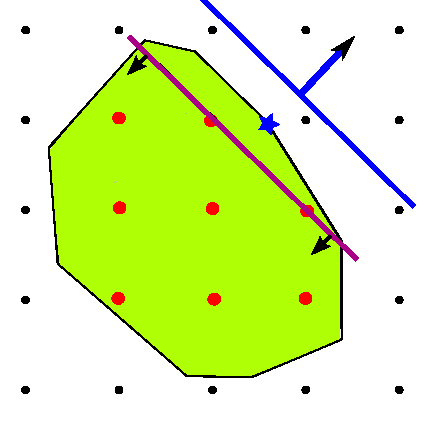
\includegraphics[scale=0.75]{CPalgorithm6.pdf}
%\end{figure}
\end{center}

\end{multicols}

\vspace{-1cm}

\subsection{How to compute cutting planes}

Two approaches:

\begin{enumerate}
	\item Computing cutting planes for general IPs.
	\begin{itemize}
		\item From ``Algebraic'' properties: CG cuts, MIR inequalities, functional cuts, etc.
		\item From ``Geometric'' properties: lattice-free cuts, etc.
	\end{itemize}
	
		\item Computing cutting planes for specific IPs.
	\begin{itemize}
		\item Knapsack problem, Node packing, etc. (many many other examples\dots)
	\end{itemize}
\end{enumerate}



\section{Computing cutting planes for general IPs}
\subsection{Chv\'atal-Gomory cuts (for pure integer programs)}

\begin{definition}[Chv\'atal-Gomory cut for $P$] Let $P\subseteq\R^n$ be a polyhedron. Let $a\in \Z^n$, $b\in \R$ and let $a^Tx\leq b$ be a valid inequality for $P$. Then the inequality
$$a^Tx\leq \lfloor b\rfloor$$
is called a Chv\'atal-Gomory cut.
\end{definition}
\begin{remark} Some examples of CG cuts are:  blossom inequalities for the matching problem, clique inequalities for the independent set problem, Gomory's fractional cut.
\end{remark}

\subsubsection{A nice property of CG cuts}

\begin{definition}[Chv\'atal-Gomory closure of $P$] Let $P\subseteq\R^n$ be a polyhedron.  Then the set
$$P'=P\ \cap\ \bigcap_{\substack{\alpha^Tx\leq\beta\\ \text{is a CG cut for $P$}}}\{x\in\R^n\tq \alpha^Tx\leq \beta\}$$
is called a Chv\'atal-Gomory closure.
\end{definition}
\begin{theorem}[Finiteness of the CG cuts procedure]
Let $P_0$ be a rational polyhedron and for $k\in\Z_+$ define $P^{k+1}=\big(P^k\big)'$. Then
\begin{enumerate}
	\item For all $k\in\Z_+$, $P^k$ is again a rational polyhedron.
	\item There exists $t\in\Z_+$ such that $P^t=P_I$.
\end{enumerate}
\end{theorem}
\subsection{Cutting planes from the Simplex tableau}
Assume $P=\{x\in\R^n\tq Ax=b,\ x\geq0\}$ where $A\in\R^{m\times n}$ is a full-row rank matrix. Let $B$,$N$ denote the basic and nonbasic variables defining a vertex $(\hat x_B,\hat x_N)$ of $P$ (where $\hat x_N=0$). You can write the constraints defining $P$ in terms of the basis $B$:
\begin{align*}
x_B&=\bar b -\bar A_N x_N\\
&x_B,x_N\geq0,
\end{align*}
where $\bar b=A_B^{-1}b$ and $\bar A_N=A_B^{-1}A_N$. 

\vspace{0.2cm}

Denote $\bar b=(\bar b_i)_{i\in B}$ and  $\bar A_N=(\bar a_{ij})_{i\in B, j\in N}$. Assume that $\bar b_i\notin \Z$, so the vertex is fractional \big(that is, $(\hat x_B,\hat x_N)\notin \in \Z^n$\big), and therefore, we would want to cut off that LP solution.

\begin{remark} Recall that the vertex $(\hat x_B,\hat x_N)$ is the only feasible point in $P$ satisfying $x_N=0$. We will use this fact in order to derive some cutting planes.
%\begin{align*}
%x_B&=\bar b \\
%x_N&=0.
%\end{align*}
%We will use this fact in order to derive some cutting planes.
\end{remark}

\subsubsection{A simple inequality}
The following is a valid inequality that cuts off the fractional vertex:
$$\sum_{j\in N}x_j\geq 1.$$
\subsection{A stronger inequality}
Let $N_f=\{j\in N\tq \bar a_{ij}\ \text{is fractional}\}$. Then the following is a valid inequality that cuts off the fractional vertex:
$$\sum_{j\in N_f}x_j\geq 1.$$
\subsubsection{Gomory's fractional cut}
The following inequality can be derived as a CG cut:
$$\sum_{j\in N}\big(\bar a_{ij}-\lfloor \bar a_{ij} \rfloor \big)x_j\geq (\bar b_{i}-\lfloor \bar b_{i} \rfloor \big).$$

It can be verified that this valid inequality cuts off the fractional vertex.



\section{Cutting planes from lattice free sets}
\subsection{ The general case}

\begin{definition}[Lattice-free sets]  {\color{blue} A set $L\subseteq \R^n$ is a lattice-free set if it does not contain any integral vector in its (topological) interior, that is, $\int(L)\cap\Z^n=\emptyset$.}
\end{definition}


Let $P$ be a polyhedron and let $L$ be a lattice-free convex set. Then, we can derive cutting planes from $L$ by using the following fact:
$$P\cap \Z^n\subseteq P\setminus \int(L).$$

Such a cutting plane is called a cutting plane derived from a lattice-free set. 
\begin{remark}
It suffice to consider only the cutting planes defining facets of $\conv(P\setminus\int(L))$ as all the cuts not defining these facets are redundant.
\end{remark}


\begin{definition}[Maximal lattice-free convex sets]  A maximal lattice-free is a lattice-free convex set that is not strictly contained in any other lattice-free convex set.
\end{definition}


Maximal lattice-free convex sets are important since they give stronger cuts, since $L'\subseteq L$ implies $P\setminus\int(L)\subseteq P\setminus\int(L')$. The following is a nice property of such sets:
\begin{theorem} $L$ is a maximal lattice-free convex set if and only if $L$ is a polyhedron satisfying certain ``simple characterization''.
\end{theorem}
\begin{remark}
The fact that all maximal lattice-free convex set are polyhedra is useful because if $L$ a polyhedron, then cutting planes for the set $P\setminus \int(L)$ are likely `easy' to obtain.
\end{remark}

\subsection{Split cuts}

A special case of a maximal lattice-free convex set is the case of split sets.

\begin{definition}[Split set, split cuts] Let $\pi\in\Z^n$ and let $\pi_0\in\Z$. Then, a split set is a set of the form
$$\{x\in\R^n\tq \pi_0<\pi^Tx<\pi_0+1\}.$$
A split cut is a any cutting plane valid for $P\setminus S$, where $S$ is some split set. 
\end{definition}


\begin{remark}
The set $P\setminus S$ can be seen as a disjunction. Let $S=\{x\in\R^n\tq \pi_0<\pi^Tx<\pi_0+1\}$, then
$$P\setminus S=\{x\in P\tq \pi^Tx\leq \pi_0\} \cup \{x\in P\tq\pi_0 +1\leq  \pi^Tx\}.$$

In general, disjunctions as the one given by a split set or more general ones are very useful to derived cutting planes for integer programs.
\end{remark}

\section{Mixed-integer rounding cuts (MIR)}
\subsection{Basic MIR inequality}\label{basicMIR}
Let $B=\{(u,v)\in \Z\times \R\tq u+v\geq b,\ v\geq0\}$. Then the inequality
$$v\geq \big(b-\lfloor b \rfloor\big)\big(\lceil b\rceil - u\big)$$
is valid for the set $B$.
\subsection{MIR inequalities from one-row relaxations}
Let $P$ be a polyhedron. We want to find valid inequalities for $P\cap (\Z^{|I|}\times \R^{|J|})$. 
\subsubsection{One-row relaxation}
A set of the form 
$$Q=\Big\{(x,y)\in \R^{|I|}\times \R^{|J|}\tq \sum_{i\in I}a_ix_i+\sum_{j\in J}c_jy_j\geq b,\ x,y\geq0\Big\}$$ 
is a one-row relaxation of $P$ if $P\subseteq Q$. 
\begin{remark}
One-row relaxations can be constructed by using any valid inequality for $P$. In particular one could obtain a valid inequality by combining rows of the matrix  and vector defining $P$.
\end{remark}
\subsubsection{Applying the basic MIR inequality}
We first relax the inequality defining $Q$. Let $I'\subseteq I$ and  consider the following mixed-integer set:
$$B=\bigg\{(x,y)\in \Z^{|I|}\times \R^{|J|}\tq\Big(\sum_{i\in I\setminus I'}x_i + \sum_{i\in I}\lfloor a_i\rfloor x_i\Big)+\Big(\sum_{i\in I'}(a_i-\lfloor a_i\rfloor)x_i+ \sum_{j\in J}\max\{0,c_j\}y_j\Big)\geq b\bigg\}.$$
Sicne the first part of the l.h.s. of the inequality is integral and the second part is nonnegative, we can apply the procedure described in Section \ref{basicMIR}. We obtain the following valid inequality for $B$:
$$\Big(\sum_{i\in I'}(a_i-\lfloor a_i\rfloor)x_i+ \sum_{j\in J}\max\{0,c_j\}y_j\Big)\geq \big(b-\lfloor b \rfloor\big)\bigg(\lceil b\rceil - \Big(\sum_{i\in I\setminus I'}x_i + \sum_{i\in I}\lfloor a_i\rfloor x_i\Big)\bigg).$$
\begin{remark}
The above inequality is valid for $P\cap (\Z^{|I|}\times \R^{|J|})$, for all $I'\subseteq I$. The set $I'=\{i\in I\tq (a_i-\lfloor a_i\rfloor)<(b-\lfloor b\rfloor)\}$ gives the strongest inequality of this form.
\end{remark}

\section{Gomory Mixed-integer cut (GMI)}
Consider the one-row relaxation $Q=\{(x,y)\in \Z^{|I|}\times \R^{|J|}\tq \sum_{i\in I}a_ix_i+\sum_{j\in J}c_jy_j= b,\ x,y\geq0\}$. Denote $f_0=b-\lfloor b\rfloor$ and for $i\in I$ denote $f_i=a_i-\lfloor a_i\rfloor$. 

We will assume that $0<f_0<1$. In this case, the Gomory mixed-integer cut (GMI) is given by
$$\sum_{\substack{i\in I\\f_i\leq f_0}}\frac{f_i}{f_0}x_i + \sum_{\substack{i\in I\\f_i> f_0}}\frac{1-f_i}{1-f_0}x_i+\sum_{\substack{j\in J\\c_j>0}}\frac{c_j}{f_0}y_j+\sum_{\substack{j\in J\\c_j<0}}\frac{c_j}{1-f_0}y_j\geq 1.$$

\begin{remark}
\text{ }
\begin{itemize}
	\item The validity of GMI cuts follows from the fact that they are also split cuts.
	\item In the pure integer programming case (that is, $J=\emptyset$), GMI gives a cut that is stronger than the Gomory's fractional cut.
\end{itemize}
\end{remark}




\includefiguresource{tikz/Illustration1.pdf}
\includefiguresource{tikz/Illustration2.pdf}
\includefiguresource{tikz/Illustration3.pdf}



\end{document}
